\documentclass[portuguese]{textolivre}

% metadata
\journalname{Texto Livre}
\thevolume{18}
%\thenumber{1} % old template
\theyear{2025}
\receiveddate{\DTMdisplaydate{2024}{12}{6}{-1}}
\accepteddate{\DTMdisplaydate{2025}{1}{14}{-1}}
\publisheddate{\today}
\corrauthor{João Alexandre Peschanski}
\articledoi{10.1590/1983-3652.2025.56372}
%\articleid{NNNN} % if the article ID is not the last 5 numbers of its DOI, provide it using \articleid{} commmand 
% list of available sesscions in the journal: articles, dossier, reports, essays, reviews, interviews, editorial
\articlesessionname{articles}
\runningauthor{Peschanski, Jurno e Hilsenbeck Filho}
%\editorname{Leonardo Araújo} % old template
\sectioneditorname{Daniervelin Pereira}
\layouteditorname{Leonardo Araújo}

\title{Emergência da extensão universitária digital: boas práticas e direcionamentos}
\othertitle{Emergence of digital university extension: best practices and guidance}

\author[1]{João Alexandre Peschanski~\orcid{0000-0002-2352-1787}\thanks{Email: \href{mailto:joalpe@wmnobrasil.org}{joalpe@wmnobrasil.org}}}
\author[1]{Amanda Chevtchouk Jurno~\orcid{0000-0002-2192-8161}\thanks{Email: \href{mailto:amandajurno@wmnobrasil.org}{amandajurno@wmnobrasil.org}}}
\author[1]{Alexander Maximilian Hilsenbeck Filho~\orcid{0009-0000-5325-3325}\thanks{Email: \href{mailto:alex.hilsenbeck@wmnobrasil.org}{alex.hilsenbeck@wmnobrasil.org}}}
\affil[1]{Wiki Movimento Brasil, São Paulo, SP, Brasil.}

\addbibresource{article.bib}

\begin{document}
\maketitle
\begin{polyabstract}
\begin{abstract}
O artigo apresenta boas práticas da Extensão
Universitária Digital. Faz um resgate histórico da prática extensionista
no Brasil, marcada por um processo gradual de institucionalização.
Indica os desafios da formação universitária, em especial de sua atuação
comunitária, na sociedade digital no Século XXI. Apresenta a crescente
orientação para que a universidade desenvolva competências
contemporâneas, incluindo o pensamento crítico, o letramento midiático,
a participação cidadã e a colaboração comunitária, afins à atuação
extensionista digital. Por meio de casos empíricos, apresenta boas
práticas da extensão universitária, com foco na soberania tecnológica,
na institucionalização de projetos e no desenvolvimento de recursos
educacionais abertos.

\keywords{Extensão universitária \sep Digitalização \sep Wikipédia}
\end{abstract}

\begin{english}
\begin{abstract}
The article highlights best practices in Digital
University Extension. It provides a historical overview of extension
practices in Brazil, shaped by a gradual process of
institutionalization. The study identifies challenges in university
education, particularly in community engagement, within the digital
society of the 21st century. It emphasizes the growing orientation for
universities to foster contemporary competencies, including critical
thinking, media literacy, civic participation, and community
collaboration, aligned with digital extension practices. Through
empirical cases, the article presents best practices in University
Extension, focusing on technological sovereignty, project
institutionalization, and the development of open educational resources.

\keywords{University extension \sep Digitalization \sep Wikipedia}
\end{abstract}
\end{english}
\end{polyabstract}


A extensão universitária é tradicional nas instituições brasileiras e os
primeiros registros de realização dessas atividades datam da década de
1910. Apesar da sua longevidade na cena educacional do Brasil,
paradoxalmente, a extensão universitária não está consolidada enquanto
prática generalizada de profissionais universitários. Indicativo disso é
a publicação de uma resolução determinando a obrigatoriedade da inserção
de atividades dessa natureza na carga horária curricular dos cursos de
graduação. Trata-se da Resolução 7, publicada em dezembro de 2018 pelo
Ministério da Educação, que instituiu as "Diretrizes para a Extensão na
Educação Superior Brasileira", além de um prazo (que se encerrou em
dezembro de 2022) para cumprimento da nova regulamentação.

Vários autores debatem sobre os motivos para a não-adesão histórica ao
modelo pedagógico extensionista e um argumento parece ser coincidente
entre eles: a falta de investimentos e priorização de financiamento
público específico para iniciativas dessa natureza
\cite{Gomez2019, Oliveira2015, Paula2013}. Diante de um cenário de
constante precarização e de crise orçamentária das universidades, além
da sobrecarga de educadores, a realização de atividades de extensão
parece ser preterida frente às atividades de pesquisa e ensino.

A implementação da obrigatoriedade da extensão, sem aumento de carga
horária docente ou financiamento específico, levou várias instituições à
adesão de formatos digitais com baixo ou zero custo. Tal decisão foi
exacerbada pela pandemia de COVID-19 que exigiu a adoção de atividades
remotas e sem risco de exposição dos estudantes. Além disso,
inicialmente, a escolha de digitalização de processos pareceu ser uma
forma de adequação às linguagens usadas pelos jovens estudantes, cada
vez mais hiperconectados. Nesse processo, muitos professores conseguiram
desenvolver trabalhos importantes, com real impacto social, através do
uso de plataformas de redes sociais e aplicativos. Mas será que
consideraram os custos dessas escolhas, ao fornecer dados e materiais
para empresas proprietárias?

Antagonistas à digitalização da extensão universitária costumam pontuar
os riscos do universo digital, pela perda de autonomia da educação, do
fazer pesquisa e ciência frente a pouquíssimas grandes
corporações\footnote{Apenas na última década tem
  ocorrido um processo de hiper concentração de infraestruturas e de
  dados informacionais nas mãos de poucas empresas proprietárias. Sendo
  apenas cinco grandes corporações -- conhecidas como as Big Five ou
  GAFAM -- que se tornaram intermediárias poderosas de nossa vida
  digital: Apple, Google, Microsoft, Facebook e Amazon
  \cite{Dijck2018}.}, e defendem que a universidade pública não deve
ser conivente com as gigantes da internet \cite{Parra2018, Zuboff2015}.
Contudo, há um temor de que tal posicionamento aumente a distância entre
professores e estudantes, além de dificultar a inserção destes no
mercado de trabalho. Qual seria então a solução para esse dilema?

Podemos pensar na perspectiva das ações de ensino, pesquisa e extensão a
partir da construção de um ecossistema informacional protegido e livre,
que garanta a segurança de dados e metadados institucionais e pessoais,
e que seja, ao mesmo tempo, seguro, consciente e eficiente, com projetos
com alto impacto educacional e social. Desse modo, urge possibilitar e
adotar soluções alternativas para a extensão universitária, que estejam
alinhadas com a hiperconectividade da sociedade e com as possibilidades
de impacto social em escala ampliada. Essa construção é possível sem
abdicar da transparência sobre os efeitos econômicos, políticos e
sociais da adoção das tecnologias e infraestruturas sociotécnicas
utilizadas na educação, na pesquisa científica e na extensão
universitária. Em última instância, vale ressaltar que a internet não se
resume às grandes plataformas digitais proprietárias.

Pretendemos demonstrar algumas dessas potencialidades no decorrer desse
artigo.



\section{A extensão universitária - histórico e atualidade}
As primeiras manifestações do que se compreende como extensão
universitária datam da segunda metade do século XIX, na Inglaterra.
Alguns autores referem-se a um tipo arcaico de extensão universitária
surgido nas universidades medievais que realizavam atividades religiosas
e filantrópicas, representando uma fase pré-extensionista caracterizada
pelo assistencialismo \cite{Oliveira2015}\emph{.} Acredita-se que tenha
sido em 1871 que a Universidade Cambridge criou o primeiro programa
formal de cursos de extensão \cite{Paula2013}, buscando "instruir
tecnicamente as camadas populares que não tinham acesso às
universidades, suprindo as demandas da indústria em crescimento''
\cite[p.~10]{Oliveira2015}.

A partir de então, a extensão percorreu o continente europeu e chegou
aos Estados Unidos. Com a criação da \emph{American Society for the
Extension of University Teaching}, as atividades de extensão foram
impulsionadas no país, inicialmente na Universidade de Chicago (em
1892), e culminaram com a bem sucedida experiência desenvolvida pela
Universidade de Wisconsin (em 1903). Esta "conferiu prestígio e
visibilidade nacional ao que seria chamado \emph{Wisconsin Idea''}
\cite[p.~7]{Paula2013} ao colocar os professores como expertos técnicos
do governo e criar um modelo de interação com a comunidade implicando a
universidade no desenvolvimento tecnológico nacional.

Para \textcite[p.~9]{Paula2013}, a extensão universitária é "coetânea e produto
de um momento particularmente crítico da história do capitalismo" quando
se exacerbaram contradições sociais, com a entrada em cena de segmentos
historicamente marginalizados e submetidos ao capital. Na tentativa de
manutenção desta ordem, tornou-se necessária a realização de políticas
capazes de "atender/neutralizar reivindicações operário-populares"
(\emph{ibidem, }p.~9). Segundo o autor, a extensão universitária nos
países do capitalismo central pode ser dividida em duas vertentes: a
europeia (originada na Inglaterra), que se caracteriza pelo engajamento
da universidade na oferta de "contrapontos às consequências mais
nefastas do capitalismo'' (\emph{ibidem, }p.~9); e a estadunidense, cujo
principal objetivo é "a mobilização da universidade no enfrentamento de
questões referentes à vida econômica no sentido da transferência de
tecnologia, da maior aproximação da universidade com o setor
empresarial" (\emph{ibidem, }p.~9).

Na América Latina, a extensão surge protagonizada por estudantes, com
caráter de ação revolucionária, e em um contexto de luta contra o
anacronismo e a obsolescência das universidades tradicionais do período
colonial \cite{Oliveira2015,Paula2013}. Polarizado por duas
grandes revoluções --- mexicana (1910) e cubana (1959) ---, tal contexto
estabelece uma variada gama de reivindicações e lutas sociais que se
iniciam a partir da centralidade da luta pela terra e avançam para
incorporar questões sociais mais amplas \cite{Paula2013}. A partir das
demandas estudantis, de maior aproximação e interação com professores, e
do exercício do papel social da universidade, foram sendo articuladas as
concepções que viriam a fundamentar a extensão universitária,
contribuindo para seu processo de institucionalização na América Latina
e formulação de políticas públicas nesse sentido \cite{Gomez2019}. Ao
longo do processo histórico em que se desenvolveu, o caráter latino de
transformação social influenciou fortemente as ideias que constituem a
atual fase da extensão universitária brasileira \cite{Oliveira2015}.

Para compreender o caso brasileiro, caracterizado "por contradições
herdadas de sua recente história" \cite[p.~24]{Carbonari2007} e
criticado por seu caráter "assistencialista, paternalista e domesticador
de comunidades'' (\emph{ibidem, }p.~25), faz-se importante considerar a
relativamente recente implantação das instituições universitárias no
país (início do Século XX), compostas e destinadas às camadas mais
abastadas da sociedade, e a inserção destas no quadro político
institucional \cite{Gomez2019}. As primeiras iniciativas extensionistas
datam da década de 1910, na então Universidade Livre de São Paulo. Entre
1911 e 1917, foram organizados eventos abertos ao público nos quais se
discutiam diversas questões não relacionadas às problemáticas sociais e
políticas da época. Realizadas inicialmente em São Paulo, depois no Rio
de Janeiro, em Viçosa e em Lavras, as atividades foram influenciadas
tanto pelo modelo europeu quanto pelo estadunidense
\cite{Carbonari2007, Oliveira2015, Paula2013}.

A primeira referência legal à extensão universitária realizada em
território nacional se encontra em um Decreto de 1931, que trata do
Estatuto das Universidades Brasileiras \cite{Oliveira2015}. A partir
dele, a extensão se tornou um meio de divulgação da universidade por
meio da "prestação de serviços em detrimento de sua postura política"
(\emph{ibidem, }p.~12), caracterizando o que \textcite{Oliveira2015}
chamam de primeira fase/face da extensão brasileira. Acompanhando as
transformações que se deram ao longo do século XX, com o passar do tempo
alteraram-se também as orientações e a compreensão do que se configura
como uma atividade de extensão. De acordo com os autores, a segunda
fase/face desse processo, a época do assistencialismo, era composta por
projetos que "visavam ao ideal de desenvolvimento e segurança nacional
promovido pelo governo militar" (\emph{ibidem, }p.~12), pensando nos
estudantes como meros executores de tarefas.

Para compreender o que os autores chamam de terceira fase/face da
extensão, a dialógica, a obra ``Extensão ou Comunicação'' de \textcite{Freire2013} é peça central. Nela, Freire propôs um formato que visasse
comunicar conhecimentos e não transmitir conteúdos. A fase dialógica
teve grande influência das atividades extensionistas realizadas de forma
independente por jovens reunidos na União Nacional dos Estudantes (UNE)
ainda durante a ditadura militar. Os movimentos culturais e políticos
organizados pela UNE propunham a inserção do estudante na vida
comunitária e foram fundamentais para a institucionalização da extensão
universitária, por meio da demonstração do compromisso social e da busca
por uma atuação interprofissional por meio de metodologias que
possibilitassem a reflexão sobre sua prática \cite{FORPROEX2012a}.

Na década de 1980, as universidades buscaram acompanhar o projeto
nacional democrático e a extensão passou a ser um espaço de realização
de práticas que assegurassem os direitos humanos \cite{Carbonari2007}.
A partir das lutas de reconstrução das instituições políticas e sociais,
ocorreu a redefinição das práticas relacionadas ao Ensino, Pesquisa e
Extensão e a reformulação da concepção de Universidade Pública,
questionando-se a visão assistencialista das ações extensionistas. Com a
criação do Fórum de Pró-reitores de Extensão das Instituições de
Educação Superior Públicas Brasileiras (FORPROEX), em novembro de 1987,
os Pró-Reitores das universidades públicas começaram a se reunir para
debater conceitos e políticas extensionistas. Nesse fórum foi aprovado o
Plano Nacional de Extensão (PNE), de 1998, ganhando espaço na
Constituição Federal Brasileira de 1988 e na Lei de Diretrizes e Bases
da Educação de 1996, institucionalizando e formalizando a extensão
universitária, que passou a ser considerada indissociável do ensino e da
pesquisa \cite{Gomez2019}. A partir de então, a extensão superou a
ideia de disseminação de conhecimento, prestação de serviços e
assistencialismo, assumindo um caráter dialógico e comprometido com a
transformação social.

A partir da sistematização das reflexões realizadas no FORPROEX, em 2012
o Plano Nacional de Extensão foi transformado na Política Nacional de
extensão universitária (PNE), documento que consolidou conceitos e
apresentou diretrizes para propostas na extensão universitária
\cite{Gomez2019}. A PNE buscou reafirmar os objetivos pactuados ao
longo da existência do Fórum, acrescentando outros considerados
fundamentais para o "enfrentamento de novos desafios e aproveitamento de
novas oportunidades" \cite{FORPROEX2012a}. No início dos anos 2000, a
extensão universitária já dispunha de significativa densidade
institucional, sendo considerada o "instrumento por excelência de
inter-relação da Universidade com a sociedade" (\emph{ibidem}), capaz de
possibilitar a oxigenação, a democratização e a reprodução do
conhecimento acadêmico através da troca de saberes com as comunidades.

Ao inaugurar a exigência de creditar no mínimo 10\% da carga horária da
graduação a projetos ou programas de extensão, em áreas de pertinência
social, os Planos Nacionais de Educação \cite{Brasil2001} também
contribuíram para esse processo de institucionalização. Contudo, autores
como \textcite[p.~7]{Gomez2019} destacam a contradição da
inexistência de priorização de financiamento público específico para
iniciativas dessa natureza, prejudicando seu desenvolvimento em um
cenário de "contingenciamento de recursos financeiros" no orçamento das
universidades. Em 18 de dezembro de 2018, foi publicada a Resolução nº 7
do Ministério de Educação com o objetivo de estabelecer diretrizes para
a curricularização da extensão na Educação Superior Brasileira,
determinando que as Instituições de Ensino incluíssem tais atividades na
matriz curricular da graduação \cite{Brasil2018}. O prazo para a
adaptação e implementação das novas Diretrizes se encerrou em dezembro
de 2022, após extensão concedida em função da pandemia da COVID-19
\cite{Brasil2020}.

De acordo com o \textcite{FORPROEX2019}, via "Mapeamento da Inserção da Extensão
nos Currículos dos Cursos de Graduação das Instituições Públicas de
Educação Superior Brasileiras" (IPES), publicado no início de 2019, a
maioria das instituições deu início aos processos de debate e
implantação das novas diretrizes da extensão em cumprimento às metas do
PNE 2014-2024, antes mesmo da publicação da resolução 07/2018/CNE/MEC.
Contudo, esta impactou o ritmo e a forma de condução do tema, auxiliando
a convencer comunidades e gestões acadêmicas, amparando legalmente as
decisões e determinando a aceleração dos processos em instituições que
ainda não haviam iniciado a construção de normativas internas. O
mapeamento em questão contou com a participação de cerca de 70 IPES e
permitiu compreender a importância dada à temática.

Somada à gradativa institucionalização, a história da extensão
universitária também é marcada pela sua massificação, tanto em relação
ao número de instituições participantes, quanto ao impacto das
atividades realizadas. Em 1987, registrou-se a participação de 33
instituições durante o primeiro Encontro de Pró-Reitores de Extensão das
Universidades Públicas Brasileiras \cite{FORPROEX1987}. Em 2023, foram
registradas 160 instituições Federais, Estaduais e Municipais membros do
FORPROEX \cite{RENEX2016}. De acordo com o Censo da extensão
universitária, ao longo de 2022 foram realizadas cerca de 114 mil
atividades, envolvendo 190 mil professores e mais de 2 milhões de
estudantes extensionistas \cite{RENEX2023}. Além disso, mais de 680 mil
professores da rede pública foram contemplados nessas iniciativas, que
contaram com 140 milhões de pessoas participantes.

Conforme a PNE, o "quadro sombrio" contemporâneo é composto por uma
crise civilizatória expressa na inter-relação e interdependência de
várias outras crises. Vivenciamos crise ambiental e urbana, crise do
emprego, crise do Estado de Bem-Estar e da administração burocrática,
crise energética, econômica e também cultural. Acrescentamos a essas, as
crises informacional e de legitimidade da ciência que assolaram o mundo
nos últimos anos.


\section{Formação para o século XXI e o papel da extensão}

As transformações impulsionadas pelo avanço da tecnologia digital em uma
sociedade em rede \cite{Castells1999} compeliram mudanças e
reestruturações no ``mundo do trabalho'', exigindo diferentes
habilidades profissionais, mas também uma reconfiguração das relações
sociais. Com a abertura desse mundo contemporâneo, novas contradições
são postas em cena, provocando diretamente a formação educacional em
seus distintos níveis, sobretudo em um cenário cada vez mais
globalizado, digital e em constante transformação.

Objetivando incidir na integração de habilidades e competências a serem
desenvolvidas no ensino, uma aliança organizada em 2002, em torno da
Organização das Nações Unidas para a Educação, Ciência e Cultura
(UNESCO) --- a "\emph{Partnership for 21st Century Learning"} (P21) ---
desenvolveu uma estrutura para a aprendizagem chamada de ``Habilidades
para o século XXI'', que defende uma abordagem integrada na educação,
com habilidades cognitivas, sociais e digitais. Esse documento apresenta
uma série de competências e disposições de aprendizagem identificadas e
formuladas por educadores, empresários, acadêmicos e agências
governamentais, que estes consideraram fundamentais para o ``êxito'' dos
estudantes no trabalho e na vida, na tentativa de alinhamento da
educação e do desenvolvimento de pessoas com as demandas societárias
contemporâneas e futuras \cite{Dede2009}.

Outro marco na definição das competências e habilidades para o século
XXI é o documento \emph{Education 2030 Framework for Action} da UNESCO
\cite{UNESCO2016}, realizado em conjunto com outras instituições
globais que organizaram o Fórum Mundial de Educação 2015, na Coréia do
Sul, que reuniu representantes de 160 países, entre ministros, chefes de
Estado, representantes da sociedade civil e de setores privados, para
discutir perspectivas educacionais para os próximos 15 anos. O documento
destacou uma educação que abranja competências cognitivas e habilidades
socioemocionais, com foco na sustentabilidade e cidadania global.

De modo geral, entre os diversos grupos que desenvolvem conceituações de
habilidades do século XXI, identifica-se uma tendência de cenário do
mundo do trabalho com ênfase nas rápidas transformações tecnológicas e
sociais. Consideram necessárias novas habilidades dinâmicas para a
adaptação, destacando a colaboração, empatia, raciocínio abstrato,
resiliência e ética como competências fundamentais a serem desenvolvidas
na educação. Nota-se que grupos dão diferentes destaques para áreas mais
específicas dentro do conjunto mais abrangente de habilidades
\cite{Dede2009}.

A presença e a tentativa de confluência dos interesses empresariais e
sociais na educação não são novidades. As questões envolvendo trabalho e
educação passam por revisões conforme os arranjos regionais dos poderes
políticos e econômicos são delineados. Contudo, a ampliação da presença
empresarial na educação se intensificou no início da década de 1970, em
nome da ``luta contra o déficit da escola''. Conjuntamente, revigorou a
aprendizagem na empresa, acirrando a disputa com valores republicanos
que privilegiam a escola como espaço para formação de cidadãos. Nas
últimas décadas, a associação entre as noções de ``competência'' e
``saber'' avançou nas dimensões escolar e profissional, gerando forte
impacto na reorganização de currículos escolares e acadêmicos, e também
nas formas de integração do trabalhador no mercado de trabalho
\cite{Segnini2023}.

Em grande parte das vezes, ``competência'' e ``saber'' são usados de
modo polissêmico e vago, permitindo a neutralização de contradições
sociais na popularização dos seus usos. De acordo com \textcite{Rope1997}, a implementação e difusão no uso desses termos visa a mudança de
um sistema de ensino centrado sobre os saberes no centro de ramificações
escolares para um sistema de aprendizagem centrado no estudante, ator de
sua trajetória escolar, passando-se de uma organização produtiva na qual
podia-se (ou não) desenvolver uma carreira para uma organização
valorizante criadora de competências para o indivíduo assalariado
(\emph{ibidem}). Em ambos os casos, observa-se uma busca obstinada pela
individualização, num processo alinhado com transformações sociais
decorrentes do avanço tecnológico e comunicacional. Isso leva a mudanças
profundas na reorganização do mundo do trabalho e em seus modos de
gestão, além das relações sociais e formas de subjetivação dos
indivíduos na sociedade\footnote{Temos que
  contextualizar, em cada país e localidade, o processo próprio de
  regionalização das políticas educacionais e as distintas escalas da
  relação entre trabalho e educação, por vezes com forte presença das
  federações patronais na disseminação de propostas (como se observa em
  tempos neoliberais, com o glossário das políticas públicas tendo o
  termo onipresente de \emph{empreendedorismo} no ambiente escolar e
  forte responsabilização individual na inserção no mundo do trabalho),
  ocorrendo, em cada caso, maior ou menor aval e apoio político e
  financeiro do Estado.}.

A educação e o debate sobre seus novos modos de gestão inserem-se como
objeto de disputa atual associado às particularidades do nosso tempo. O
processo de ensino-aprendizagem se incorpora a uma lógica em que a
competitividade econômica individual irrompe como uma das principais
catalisadoras de nosso sistema, e num campo cuja existência de
indicadores de aprendizagem nas escolas reflete uma mensuração com
vistas ao desenvolvimento de habilidades voltadas às necessidades do
mercado de trabalho. Para tal, a formação e a educação são associadas
para estabelecer valores voltados ao empreendedorismo, por meio de
ideias vinculadas a um trabalhador flexível no decorrer do percurso
formativo. Contudo, esse é um processo contraditório, pois trata-se de
formas de pensamento e organização social por vezes antagônicas, com
pretensões de abarcar as maiores dimensões da vida individual e social.

O empreendedorismo como padrão social associa-se, no digital, às
práticas anticomunitárias, no sentido de não promoverem o bem comum.
Assim, o debate público digital torna-se um campo em que se desenvolvem
o negacionismo, o revisionismo e a desinformação
\cite{Anthonysamy2022, Ciampaglia2018}. Atuar nos ambientes digitais de
forma consciente e intencionada, em prol de práticas comunitárias, é
fundamental para promover valores ligados ao ensino transformador que
pretende a universidade.

No caso brasileiro, têm impacto sobre a educação digital as
características próprias de uma sociedade com desigualdades
correspondentes ao seu tamanho continental. Contudo, alguns aspectos
gerais merecem ser destacados. Em pesquisa publicada em junho de 2024,
pela Organização para Cooperação e Desenvolvimento Econômico (OCDE), e
realizada pelo instituto \emph{Truth Quest} em 21 países, foi simulada
uma rede social onde os participantes deveriam classificar as notícias
(The OECD {[}...{]}, 2024). O Brasil obteve o pior índice na capacidade
da população adulta em identificar conteúdo falso e enganoso online.
Somado a essa situação, dados do PNAD-C apontam que, em 2022, somente
39\% dos domicílios brasileiros acessaram serviços digitais do governo,
sobretudo porque as pessoas não possuem as habilidades necessárias para
tal \cite{Mahdi2024}. De acordo com o \emph{World Skills Clock}
\cite{ONU2024}, as habilidades digitais no Brasil não estão muito
disseminadas entre os jovens do país, fazendo com que o Brasil esteja na
119ª posição de 168 nações em relação à proporção de jovens com
habilidades digitais. Nos resultados do último Pisa (Programa
Internacional de Avaliação de Alunos) --- que mede conhecimentos de
estudantes de 15 anos --- apenas 2\% dos jovens brasileiros atingiram os
níveis mais altos de proficiência em leitura. Tais dados demonstram a
dificuldade da população brasileira de diferenciar fatos de opiniões e,
portanto, distinguir conteúdos falsos e verdadeiros, sendo o ambiente
digital um terreno fértil para disseminação de desinformação e
\emph{fake news}.

Tais dados demonstram a necessidade urgente de inserir o letramento
midiático como parte da formação cidadã dos estudantes. Portanto, ocupar
o espaço digital de forma consciente e ativa, através da implementação
de educação midiática e comunicacional, que permita o acesso à
informação de forma analítica e crítica, além da criação de conteúdos de
modo ético e responsável, se torna fundamental para o desenvolvimento de
uma sociedade melhor, o que é parte do papel da universidade pública.

Competências cognitivas (como pensamento crítico, criatividade,
resolução de problemas), de informação, na interface de mídia e
tecnologia (letramento midiático, informacional e comunicativo), e
sociais e emocionais (colaboração e comunicação) podem servir de
horizonte para o desenvolvimento da formação estudantil. Tais
competências provêm as ferramentas necessárias para que os estudantes
possam analisar criticamente cenários e diferentes vieses da construção
da informação, potencializando os resultados para além da comunidade
escolar e abarcando a sociedade de modo mais geral. Isso pode ser
fomentado por projetos e atividades extensionistas digitais através de
ferramentas e plataformas livres, que atuam na construção do
conhecimento e da ciência aberta.

Na contemporaneidade o mundo digital já faz parte do ambiente público.
Não podemos escapar de sua ubiquidade, tampouco do papel que todas as
formas de tecnologias de informação e comunicação (TIC) desempenham em
nossa vida pessoal, econômica, política e social. Assim, cobra
relevância o documento da UNESCO sobre alfabetização midiática e
informacional e o currículo para formação de professores, que defende
que novas formas de competências --- isto é, conhecimentos, habilidades
e atitudes --- são necessárias para que as pessoas efetivamente
participem nas sociedades da informação e do conhecimento, sendo capazes
de usufruir das liberdades fundamentais e da prática de autodeterminação
e desenvolvimento. O papel da qualidade, fiabilidade e disponibilidade
da informação online se faz decisivo, pois baliza as capacidades de
escolhas e de ações (\emph{ibidem}), o que se relaciona ao usufruto dos
direitos fundamentais à liberdade de expressão e à informação, expressos
no Artigo 19 da Declaração Universal dos Direitos Humanos
\cite{ONU2019}. Nesse ponto, também pode atuar a universidade em seu
papel de produtora e disseminadora de conhecimento científico, confiável
e relevante, compartilhando na internet o resultado da curadoria
informacional e das pesquisas desenvolvidas internamente para acesso da
população geral.

\section{Orientações para interessados na extensão universitária digital}

A extensão universitária digital visa assegurar que as práticas
cotidianas, como o uso de plataformas tecnológicas, sejam qualificadas
no contexto educacional. São conhecidos os riscos do uso de dispositivos
em sala de aula, como a promoção do vício e da distração digital, a
ampliação do \emph{cyberbullying}, a sensação de vigilância combinada à
violação de privacidade no processo de ensino e aprendizagem, bem como a
dependência em relação a plataformas comerciais \cite{Selwyn2020}. Mas
desdenhar ou, ainda mais gravemente, banir o uso da tecnologia digital
no ambiente educacional é contraproducente, pois ignora a transformação
do espaço universitário, agora um híbrido entre a experiência local e o
compartilhamento digital, impactando também as práticas extensionistas.
O banimento, em particular, cria uma desconexão entre a experiência
universitária e a realidade altamente tecnológica dos estudantes,
falhando em auxiliá-los a lidar com as novas configurações da sociedade
em que vivem, além de desperdiçar as potencialidades das tecnologias
digitais para o desenvolvimento da extensão.

A promoção de práticas universitárias digitais, incluindo a extensão,
pode melhorar a qualidade da internet em português e, com isso, garantir
que a universidade atue no espaço público tal qual ele se configura
contemporaneamente, altamente digitalizado. Sem uma atuação
universitária consistente, o espaço público digital pode estimular e
caracterizar-se pela promoção do negacionismo, revisionismo e
desinformação \cite{Anthonysamy2022, Ciampaglia2018}. A extensão
universitária foi criada e evoluiu com a missão de abrir à sociedade o
conhecimento produzido e curado no ambiente acadêmico e, com a
digitalização social, é natural que ocorra também a evolução tecnológica
das práticas extensionistas e a viabilização da riqueza das redes.

A fim de potencializar as oportunidades da transformação digital da
extensão universitária, é possível seguir algumas orientações e
direcionamentos, baseados em experiências variadas. Esta seção coloca em
evidência boas práticas na extensão universitária digital, de acordo com
a soberania tecnológica, a institucionalização e a aderência às práticas
educacionais abertas, tendo como pano de fundo o desenvolvimento de
habilidades formuladas e destacadas como fundamentais para a inserção
profissional dos jovens na sociedade contemporânea e para a efetividade
da cidadania, conforme descrito no item anterior. A seguir, trazemos
alguns exemplos com objetivo de ilustrar boas práticas, sem a
expectativa de que seja um levantamento sistemático e exaustivo,
separados em três tópicos: "Soberania tecnológica",
"Institucionalização" e "Práticas educacionais abertas".

\subsection{Soberania tecnológica}

O colonialismo digital refere-se à prática de depender tecnologicamente
de dispositivos, protocolos de rede, linguagens de programação e
softwares de grandes empresas. As \emph{big techs}, empresas que dominam
o mercado digital, concentram um controle desproporcional sobre a
infraestrutura e as ferramentas digitais essenciais \cite{Avelino2021}.
Isso cria um cenário em que as instituições e usuários são
frequentemente submetidos às suas condições e limitações, estabelecendo
um modelo de dependência. Esse fenômeno resulta em uma forma de
dominação que limita a autonomia e a inovação, além de comprometer a
privacidade e a segurança dos dados ao manter a posse e o controle
centralizado nas mãos dessas corporações \cite{Amadeu2021}.

A soberania digital refere-se à capacidade de um país, instituição ou
indivíduo de controlar e proteger seus dados e sistemas digitais sem
depender de tecnologias proprietárias que possam comprometer sua
autonomia (D'Almonte; Santos, 2024). Softwares livres e recursos
educacionais abertos são normalmente considerados pilares da soberania
digital, na medida em que permitem direitos básicos a quem os utiliza:
de reter conteúdo, por meio de cópias ou armazenando-o em um dispositivo
pessoal; de reutilizar o material em diferentes contextos, como em
ambientes educacionais ou em produtos midiáticos; de revisar, que inclui
adaptar, ajustar e modificar o conteúdo, como a tradução para outro
idioma; de remixar, que envolve combinar o conteúdo original com
material revisado ou outros recursos para criar algo novo; e o direito
de redistribuir, que permite compartilhar cópias do conteúdo original e
das obras derivadas. Softwares livres e recursos educacionais abertos
têm um impacto potencialmente estruturante e viral, pois os direitos que
o definem estabelecem a base para o compartilhamento de conhecimento
comum e exigem que as obras derivadas sejam compartilhadas sob uma
configuração jurídica compatível \cite{Benkler2005}.

As universidades públicas brasileiras, ao lidarem com a crescente
digitalização e o uso de tecnologias de informação, muitas vezes acabam
servindo à lógica colonial de exploração de dados. De acordo com
pesquisa realizada em 2020, 65\% das Universidades Federais Brasileiras
possuíam contrato com Google e/ou Microsoft \cite{Mian2021}. Tal
"capitalismo universitário" \cite{Santos2018} se manifesta quando essas
instituições, ao adotar plataformas e serviços de grandes corporações
tecnológicas, não apenas transferem a gestão e a análise de dados
críticos para essas empresas, mas também perpetuam um ciclo de
dependência tecnológica no uso de programas básicos, como correio
eletrônico, repositório e outras tecnologias. O controle centralizado
exercido por essas corporações sobre as ferramentas e plataformas
utilizadas pode levar à apropriação de dados acadêmicos e pessoais,
restringindo a autonomia das universidades e potencialmente expondo
informações sensíveis a práticas comerciais e políticas externas. Também
determinam e engessam as possibilidades existentes conforme o que
funciona melhor para o modelo de negócio dessas corporações
\cite{Cassino2021}.

A atuação digital universitária, em especial na extensão, pode atuar
como uma alternativa ao colonialismo digital ao promover a autonomia
tecnológica e a soberania digital. Por um lado, as universidades podem
desenvolver e adotar soluções próprias, como plataformas de código
aberto e ferramentas de gestão de dados locais. Por outro lado, podem
selecionar soluções tecnológicas que atendam a critérios elevados de
soberania digital. A adoção de práticas digitais livres nas
universidades, em especial na extensão, pode fomentar a criação de
infraestruturas digitais sustentáveis e independentes, que respeitam a
privacidade e os direitos dos usuários, e que incentivam práticas
inovadoras e éticas, além de servir como espaço de instrução e incentivo
ao uso crítico das tecnologias digitais por parte dos estudantes
\cite{Mian2021}.

Um exemplo de atuação cívica apoiada por projetos universitários no
modelo de extensão é a iniciativa "Resposta às Enchentes do Rio Grande
do Sul", lançada em maio de 2024 (Enchentes {[}...{]}, 2024). Com o
objetivo de mapear as inundações que ocorreram no estado em abril do
mesmo ano, o projeto focou na criação de uma cartografia dos desastres
provocados pelas enchentes, incluindo inundações, movimentos de massa,
quedas de barreiras e destruição de pontes e estradas (\Cref{fig01}). A
tecnologia utilizada foi o OpenStreetMap, uma ferramenta de mapeamento
colaborativo em licença livre, e o projeto foi realizado por meio de uma
parceria entre organizações não governamentais e atividades
universitárias dedicadas ao mapeamento colaborativo com licença livre
\cite{Souto2024}.

\begin{figure}[htbp]
\centering
\begin{minipage}{.75\textwidth}
 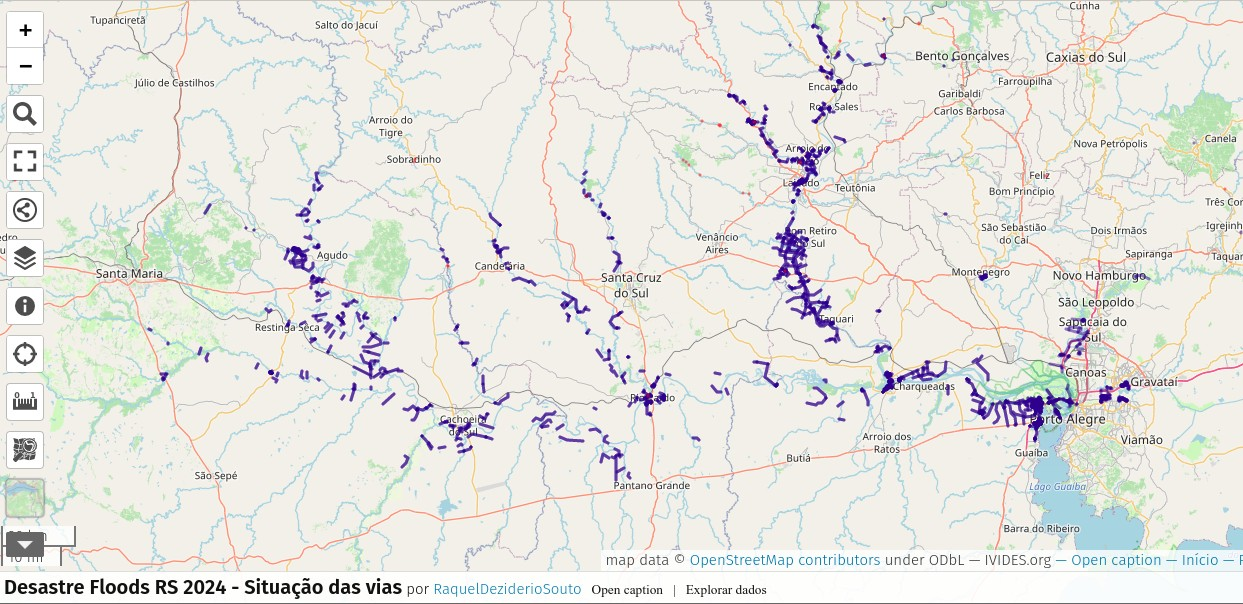
\includegraphics[width=\textwidth]{figure01.jpg}
 \caption{Imagem de uma das cartografias realizadas no projeto,
retratando as vias bloqueadas no estado do Rio Grande do Sul em junho de
2024.}
 \label{fig01}
 \source{\url{https://wiki.openstreetmap.org/wiki/File:Vias_bloqueadas_no_Rio_Grande_do_Sul_-_Situa\%C3\%A7\%C3\%A3o_em_23-06-2024.png}}
\end{minipage}
\end{figure}

Outro exemplo é a iniciativa Querido Diário que atua na intersecção
entre ciência da informação e transparência cívica, operando como
plataforma de código aberto dedicada à catalogação, descrição e
ampliação do uso de informações contidas nos diários oficiais
municipais. Esse projeto agrega dados públicos e os apresenta em uma
interface acessível, facilitando análises e usos por públicos amplos
(\Cref{fig02}). Sua natureza colaborativa catalisa parcerias significativas
com instituições de ensino superior, particularmente por meio de
projetos de extensão universitária, que proporcionam um ambiente para
que estudantes de diversas áreas do conhecimento se engajem em
atividades práticas de inovação e difusão de informações, tornando os
dados públicos acessíveis e compreensíveis (Open Knowledge Brasil,
{[}s.d.{]}).

\begin{figure}[htbp]
\centering
\begin{minipage}{.75\textwidth}
 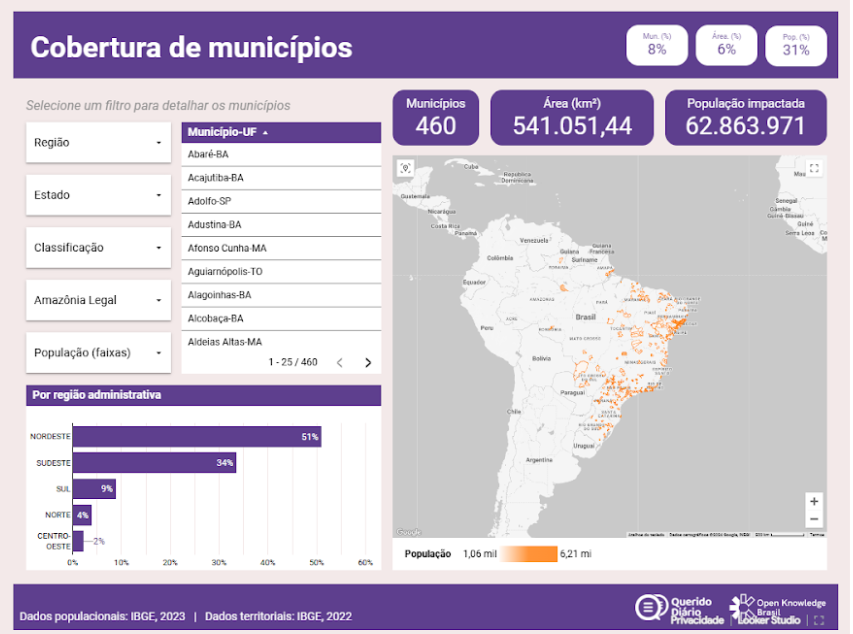
\includegraphics[width=\textwidth]{figure02.png}
 \caption{Captura de tela mostrando as cidades disponíveis no site do
projeto Querido Diário feita no dia 22 de novembro de 2024.}
 \label{fig02}
 \source{\url{https://queridodiario.ok.org.br/cidades-disponiveis}}
\end{minipage}
\end{figure}


\subsection{Institucionalização}

A manutenção sustentável de programas de extensão universitária
contribui para um ambiente de formação continuada de competências na
universidade e para um impacto social mais efetivo, em especial na
promoção de práticas inovadoras no campo digital. Um possível formato
adequado para a extensão universitária digital é o laboratório, em que
estudantes, professores e membros da comunidade podem interagir e
desenvolver competências práticas \cite{Girardi2024}. A
prática laboratorial e outras soluções continuadas dependem da
institucionalização da extensão universitária, que garante a viabilidade
dos projetos a longo prazo. Um problema que a institucionalização supre
é a apropriação mais consistente de tecnologias livres, que muitas vezes
são negligenciadas por usuários comuns de plataformas digitais.

A institucionalização da extensão universitária, em especial a digital,
também facilita a gestão de ciclos de projetos, permitindo uma atuação
progressiva e contínua. Projetos estruturados podem se beneficiar do
desenvolvimento de parcerias duradouras, por exemplo, com ONGs, como na
iniciativa sobre as enchentes no Rio Grande do Sul, o que pode aumentar
sua capacidade de impacto e alcance. O foco nas parcerias permite que,
além de resolver problemas imediatos, sejam construídas soluções sociais
sustentáveis com potencial para impacto duradouro, permitindo que os
estudantes participem de projetos com grande potencial de transformação
social.

O foco institucional coloca docentes no centro de iniciativas de
extensão universitária, que podem atuar na coordenação e continuidade
dos projetos. Podem ser um elo de facilitação e integração com
tecnologias e práticas, garantindo que as atividades estejam alinhadas
com uma missão acadêmica e comunitária. Com o risco de ir na contramão
das orientações da PNE 2012, o desafio é garantir autonomia suficiente
para discentes atuarem de modo automotivado e consciente também no
ambiente laboratorial, o que pode ser desenvolvido por meio da
realização autônoma de atividades no escopo de um projeto mais amplo.

Um exemplo de institucionalização na extensão universitária digital é o
projeto ``Reformulação e construção de verbetes da Wikipédia na área de
Teoria da História'', na Universidade Federal de Santa Catarina
\cite{Varella2020}. Dentre os objetivos da iniciativa está o de
melhorar o conteúdo sobre história na Wikipédia. O contexto foi notar
lacunas e erros em como os temas de interesse eram retratados nessa
enciclopédia eletrônica em licença livre.

O projeto teve dentre seus impactos a criação e melhoria de dezenas de
artigos, desde 2018, inclusive alguns considerados dentre os melhores na
Wikipédia, como História pública\footnote{Link do
  verbete:
  \url{https://pt.wikipedia.org/wiki/Hist\%C3\%B3ria_p\%C3\%BAblica}} e
História do tempo presente\footnote{Link do verbete:
  \url{https://pt.wikipedia.org/wiki/Hist\%C3\%B3ria_do_tempo_presente}}
(Outreach {[}...{]}, 2024). Considerando os dados referentes a essas
duas páginas, foram quase 8,5 mil visualizações nos últimos 12
meses\footnote{Dados entre Agosto de 2023 e Julho de
  2024 obtidos em
  \url{https://pageviews.wmcloud.org/?project=pt.wikipedia.org\&platform=all-access\&agent=user\&redirects=0\&start=2023-08\&end=2024-07\&pages=Hist\%C3\%B3ria_p\%C3\%BAblica\%7CHist\%C3\%B3ria_do_tempo_presente}
  no dia 30 de agosto de 2024.}. Vale destacar que existem diversos
recursos para facilitar a utilização da Wikipédia e outros projetos da
Wikimedia na extensão universitária, em especial um curso online chamado
WikiConecta (\Cref{fig03})\footnote{Link do curso:
\url{https://pt.wikiversity.org/wiki/WikiConecta}.}.


\begin{figure}[htbp]
\centering
\begin{minipage}{.75\textwidth}
 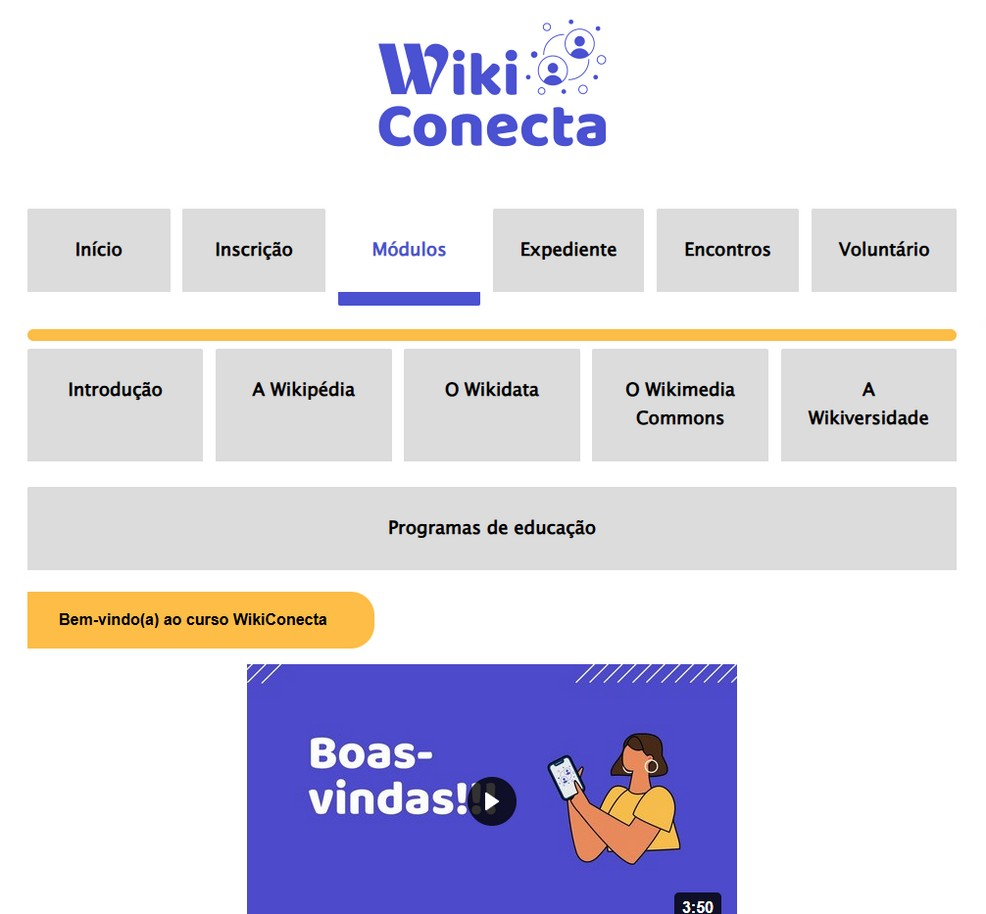
\includegraphics[width=\textwidth]{figure03.jpg}
 \caption{Captura de tela da página Módulos, mostrando o conteúdo
programático do curso aberto WikiConecta, feita no dia 26 de novembro de
2024.}
 \label{fig03}
 \source{\url{https://pt.wikiversity.org/wiki/WikiConecta/Módulos}}
\end{minipage}
\end{figure}


\subsection{Práticas educacionais abertas}

A UNESCO define os Recursos Educacionais Abertos (REAs) como ``materiais
de ensino, aprendizagem ou pesquisa que estão no domínio público ou são
liberados sob uma licença de direitos autorais que permite o uso, adoção
e distribuição gratuita do material'' \cite{UNESCO2002}. Ao estarem
disponíveis para qualquer pessoa, esses recursos possibilitam a
ampliação do acesso ao conhecimento em escala global. A licença que
adotam assegura que possam ser usados e adaptados livremente, promovendo
democratização do saber e facilitando a criação de novos materiais
educacionais.

Os REAs podem ser considerados um antídoto eficaz contra o controle do
conteúdo digital por grandes plataformas proprietárias. Dá-se o nome de
plataformização a esse controle que faz parte do processo pelo qual
plataformas digitais centralizadas, voltadas ao lucro, e altamente
escaláveis moldam e mediam a interação e a experiência do usuário. Elas
o fazem por meio de estruturas e protocolos, frequentemente invisíveis e
complexos, que influenciam a circulação e o acesso ao conteúdo em um
ambiente técnico e sociocultural específico \cite{Jurno2020}.

A permissão para que qualquer pessoa possa adaptar, compartilhar e
reutilizar o material, faz com que os REAs combatam a centralização do
conhecimento e incentivem a colaboração e a inovação na educação, além
de criar a base sociotécnica para que novos recursos sejam produzidos em
licença livre. O ecossistema que a produção e circulação de REAs fomenta
facilita conexões multidisciplinares e inter-institucionais, na medida
em que garante em algum grau segurança jurídica na utilização e
adaptação de códigos e conteúdos \cite{RamirezMontoya2020}.

As Práticas Educacionais Abertas (PEAs) incentivam a reutilização e a
criação de REAs através da implementação de políticas institucionais que
promovem o acesso e a colaboração \cite{Ehlers2011}. Dessa forma, podem
funcionar como facilitadoras da integração de modelos pedagógicos
inovadores e empoderadoras de estudantes que, pela própria configuração
da atividade, assumem o papel de pessoas co-produtoras ativas de
conhecimento, em vez de receptoras passivas. A extensão universitária
digital, tal qual proposta neste texto, se alinha às PEAs, ao adotar uma
abordagem de colaboração e compartilhamento livre de conhecimento em um
ambiente digital acessível e inclusivo.

Os Cursos Online Abertos e Massivos Conectivistas (cMOOCs) exemplificam
a aplicação de Práticas Educacionais Abertas (PEAs) no ambiente digital.
Eles disponibilizam conteúdo de qualidade e fomentam comunidades
virtuais que promovem a literacia informacional. Um exemplo notável é o
cMOOC "Introdução à Audiologia Básica" (\Cref{fig04}), hospedado na
Wikiversidade, fruto de uma colaboração interinstitucional, liderada por
Lilian Jacob, da Faculdade de Odontologia de Bauru, Universidade de São
Paulo \cite{Arrigo2024}.


\begin{figure}[htbp]
\centering
\begin{minipage}{.75\textwidth}
 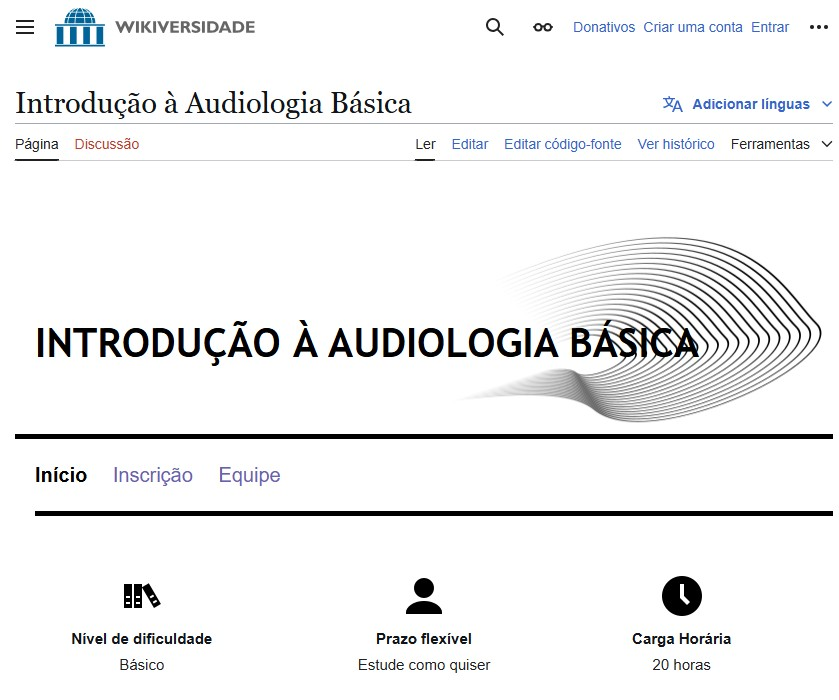
\includegraphics[width=\textwidth]{figure04.jpg}
 \caption{Captura de tela da página inicial do curso ``Introdução à Audiologia Básica'', hospedado na Wikiversidade, feita no
dia 26 de novembro de 2024.}
 \label{fig04}
 \source{\url{https://pt.wikiversity.org/wiki/Introdu\%C3\%A7\%C3\%A3o_\%C3\%A0_Audiologia_B\%C3\%A1sica}}
\end{minipage}
\end{figure}


A iniciativa visa ampliar a integridade e acessibilidade da informação
sobre audiologia em uma plataforma de alta visibilidade, atuando nos
espaços em que audiências amplas e diversas costumam procurar por
conteúdos. Isso é particularmente relevante considerando que a escassez
de conteúdo confiável contribui para a negligência nos cuidados com a
saúde auditiva \cite{Morata2024}. Ao oferecer informações precisas e
acessíveis, o curso educa sobre a temática, promove maior consciência
sobre a importância da saúde auditiva e fomenta uma comunidade virtual
de pessoas interessadas.



\section{Um novo papel para a universidade, um novo papel para a
extensão}

O objetivo deste trabalho inclui a defesa da realização de atividades
extensionistas digitais como forma de qualificar as práticas cotidianas
no contexto educacional, bem como a listagem não exaustiva de
orientações e direcionamentos que se configuram como boas práticas na
extensão universitária digital.

A extensão foi criada e evoluiu com a missão de ampliar a cultura
científica, sendo o "instrumento por excelência de inter-relação da
universidade com a sociedade" \cite{FORPROEX2012a}. Essa missão
alinha-se ao uso de tecnologias digitais, cada vez mais, onipresentes no
cotidiano hiper-conectado dos estudantes.

Entendemos que a universidade pública não pode ser conivente e manter-se
autônoma frente às gigantes da internet em um cenário de plataformização
da sociedade \cite{Dijck2018}. Contudo, justamente em um cenário
plataformizado, faz-se necessário trabalhar habilidades e competências
que possibilitem aos estudantes fazer uso consciente do digital,
preparando-os tanto para o mercado de trabalho quanto para o exercício
da plena cidadania.

Há riscos envolvendo a digitalização do aprendizado universitário. Mas,
como demonstramos ao longo deste trabalho, é possível potencializar as
oportunidades da transformação digital da extensão universitária
seguindo algumas orientações e direcionamentos de forma segura e
alinhada à missão de promoção de inter-relação com a sociedade.
Evidenciando boas práticas a partir das noções de soberania tecnológica,
institucionalização e aderência às práticas educacionais abertas,
defendemos como é possível desenvolver habilidades formuladas e
destacadas como fundamentais para a inserção profissional dos jovens na
sociedade contemporânea e para a efetividade da cidadania.

Vale destacar que enfrentamos grandes dificuldades para exemplificar
práticas alinhadas ao modelo defendido neste trabalho. Isso não
significa que tais atividades não sejam realizadas, apenas que elas não
estão documentadas academicamente e/ou não são facilmente encontradas na
internet. Essa situação demonstra que tais projetos têm impacto reduzido
às próprias redes movimentadas por eles, não sendo rastreáveis por
possíveis interessados, ou a sociedade de uma forma mais ampla.
Opostamente, o uso das ferramentas e projetos Wikimedia na realização
das atividades, insere os trabalhos em uma rede de compartilhamento
global, que conta com milhões de acessos diários, permitindo que os
estudantes vejam um impacto direto da sua atuação.


\section*{Financiamento}
A pesquisa de João Alexandre Peschanski é apoiada pela Fapesp, projeto
2013/07699-0. Agradecemos a Lucas Belo o apoio técnico. Também
agradecemos aos revisores anônimos por nos enviarem pareceres
criteriosos, que contribuíram para melhorar a forma final do texto.



\printbibliography\label{sec-bib}
%conceptualization,datacuration,formalanalysis,funding,investigation,methodology,projadm,resources,software,supervision,validation,visualization,writing,review
\begin{contributors}[sec-contributors]
\authorcontribution{João Alexandre Peschanski}[conceptualization,investigation,writing]
\authorcontribution{Amanda Chevtchouk Jurno}[investigation,writing]
\authorcontribution{Alexander Maximilian Hilsenbeck Filho}[investigation,writing]
\end{contributors}
\end{document}
